I discuss in the this section the implications in terms of architecture when porting the system from a local runtime environment to a distributed environment. The two dataflow diagrams in figure~\ref{img:dataflow_OS} and and figure~\ref{img:dataflow_Web} are used to illustrate the two cases.

\begin{figure}
    \centering
    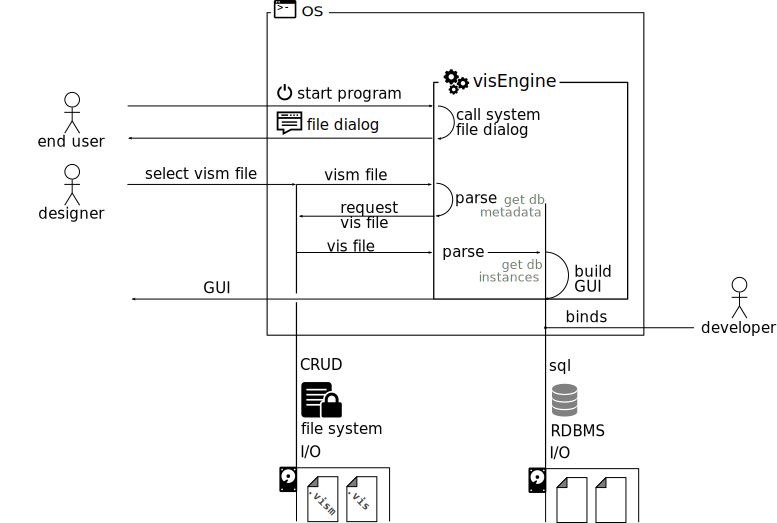
\includegraphics[angle=90,width=1\textwidth]{images/1_OS_dataflow_diagram.png}
    \caption{local runtime environment dataflow diagram}
    \label{img:dataflow_OS}
\end{figure}

\begin{figure}
    \centering
    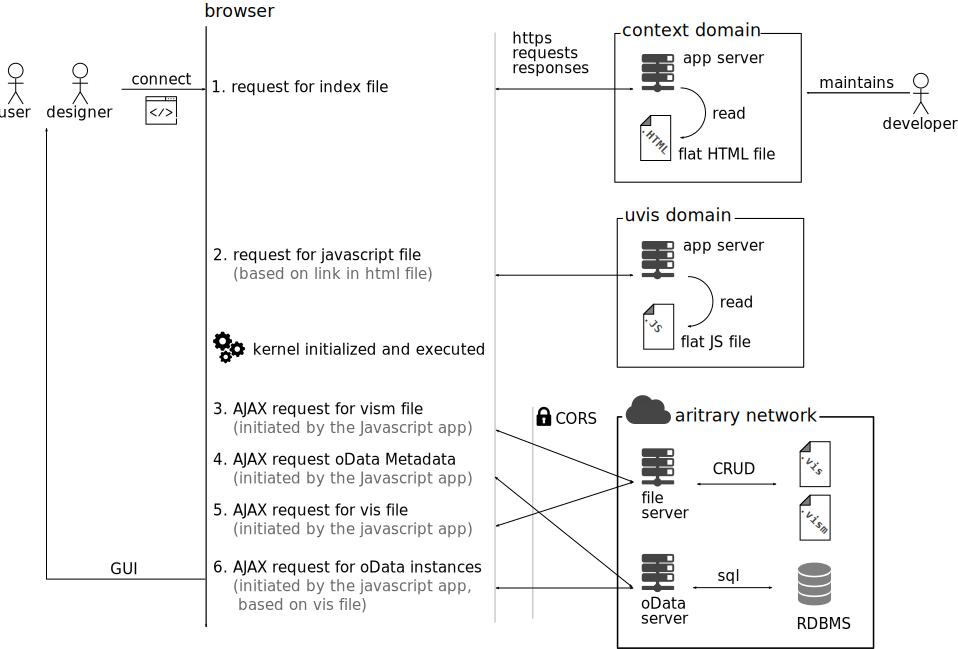
\includegraphics[angle=90,width=1\textwidth]{images/2_web_dataflow_diagram.png}
    \caption{distributed environment dataflow diagram}
    \label{img:dataflow_Web}
\end{figure}

On a local environment, end users and designers interact with the application through the computer's operating system. When starting the program, the visEngine uses the file dialog of the operating system and prompts the user for an initial vism file. Through this file dialog, the user can select any existing file on that particular file system. Note that the file system in this case is also responsible for handling the access privileges on the files. When the file is opened it's content is passed as a text stream to the engine which parses it. As described in chapter\ref{sec:description} the vism file contains the name of the initial vis file, the connection string to the database and a description of the database schema. The visEngine will first verify the connectivity to the database and thereby download the database schema which will be compared to the schema define in the file. The schema is kept in memory so that table names and table property names can be validated when addressed by the designers in the formulas. The engine will then try to find the initial vis file, on the local file system. When the file is found, the content of that file is parsed, the pre-evaluation and evaluation phases are executed and the is a result of this. In this setup, the developer's task is primarily limited to making the correct bindings to the database. Diagram~\ref{img:dataflow_OS} illustrates the architecture of the system running in a local environment.

In our case where the system is meant to run as a single page application, in a browser, and to address distributed resources across the internet, the architecture will look different. The developer's role will be extended to the maintenance of the entire domain under which the application is used. This involves at least, the maintenance and distribution of the application's shell document (the HTML page that is loaded into the browser), the configuration of the visTool application (so that it fits into the specific domain) and it's execution. From an user accessing the application as a service through the browser, the application flow will have similarities with that of a local environment, but all input/output operations of the file system on the local disk, will be replaced by actions that must be defined by the developer. Most likely these actions will be AJAX calls, triggering thereby http/tcp or https/tcp requests, but not necessarily. When an user connects to the context specific domain associated to the application, through his browser, the application's shell document is retrieved from that domain. VisTool as a javascript application is fetched in a second time, from either the context domain (where it can be cached) or directly from the uvis domain, where it is distributed as a Javascript ``bundle''. This is specified in the HTML document (written by the developer), in the ``head'' section, through a ``script'' tag (\texttt{<script src="uvis.dk/bundle.js></script>"}). Once VisTool is loaded, if started immediately the visEngine would know nothing about where and how to retrieve the initial vism file and would fail. The task of retrieving the files will depend on the context under which the application is used and is therefore also delegated to the developer. In the application's shell document the developer must also provide configuration informations for the system to use. This configuration makes the system ``context independent'' by requiring the following:
\begin{itemize}
    \item a \emph{file provider}, a method needed by the system so that it can determinate where to find the external resources (vis and vism files) based on a specific use case.
    \item an \emph{initial vism file name}, a string that is applied by our system to the fileProvider in order to retrieve the initial vismfile. As a reminder, the vism file is the starting point of the application flow. It contains amongst other the name of the visfile.
    \item a \emph{selector}, a string that represents the id attribute of a DOM element available in the current DOM tree so that our application has an element to inject it's output into.
    \item an \emph{OData client}, a string refering to an external OData client library, mainly used by our system to parse the database metadata.
\end{itemize}

The role played by the file provider is crucial in making our system decoupled from the different contexts in which it can be used. It can also be seen as a ``routing function'' that our system can rely on, at any moment, in order to apply a given resource name to an actual resource location, specific to the use context.

If the file handler method does not exist, the external resource location would have to be specified as part of the engine itself and this would require to have a different version of the system for each context of use.

Only once the application has been configured by the developer it can be started. Just like in the local version of the system, the schema described in the vism file is compared to the schema retrieved from the data service, the initial vis file is retrieved thanks to the provided file handler method, the user interface can then be generated an rendered to the user, through a HTML canvas object inserted into the browser through the DOM element whose Id attribute was provided in the application's configuration.

In this distributed architecture, the application's runtime resides within the user's browsers. In order to allow external resource to be retrieved from remote locations, the file provider method must be implemented in such a way that is handles asynchronous calls\footnote{a call is asynchronous when the result of a request for a particular resource comes as a deferred response to the current execution of the program. Since the program's execution does not await for the response, the response is typically applied to a ``callback''.  }. It is also worthwhile to note that in such a distributed environment when implementing the file provider developers will likely have to deal cross-origin HTTP requests.

A resource makes a cross-origin HTTP request when it requests a resource from a different domain than the one which the first resource itself serves. \todo[inline]{Add reference to mozilla's website here.}